\documentclass{article}
\usepackage{graphicx} % Required for inserting images
\usepackage{amsmath} % for align
\usepackage{hyperref} % Links y referencias
\usepackage{float}  % Centrar tabla donde lo puse
\usepackage{apacite}  % Citaciones en formato apa
\hypersetup{colorlinks=true, urlcolor=blue, citecolor=black, linkcolor=blue}

% Title setting
\title{Hello World!}
\author{Ian Chen}
\date{June 1, 2024}

\begin{document}
\maketitle

%%%%%%% FIRST SECTION %%%%%%%
\section{Getting Started}
\textbf{Hello World}! Today I am learning \LaTeX. \LaTeX is a great program for writing math. I can write in line math such as $a^2+b^2=c^2$. I can also give equations their own space:
\begin{align}
    \gamma^2+\theta^2=\omega^2
\end{align}
''Maxwell's equations" are named for James Clark Maxwell and are as follow:

\begin{align}
\Vec{\Delta} \cdot \Vec{E} &= \,\,\frac{\phi}{\epsilon_0}  &\text{Gauss's Law} \label{gauss1}\\
\Vec{\Delta} \cdot \Vec{B} &= \,\,0 &\text{Gauss's Law for Magnetism} \label{gauss2}\\
\Vec{\Delta} \times \Vec{E} &= \,\,-\frac{\delta \Vec{B}}{\delta t} &\text{Faraday's Law of Induction} \label{faraday1}\\
\Vec{\Delta} \times \Vec{B} &= \,\,\mu_0 \left(\epsilon_0 \frac{\delta \Vec{E}}{\delta t} + \Vec{J}\right) &\text{Ampere's Circuital Law} \label{ampere1}
\end{align}

Equations \ref{gauss1}, \ref{gauss2}, \ref{faraday1} and \ref{ampere1} are some of the most important in Physics.

%%%%%% Second Section %%%%%%
\section{What about Matrix Equations?}

\[
% Square matrix
\left(
\begin{array}{cccc}
     a_{11} & a_{12} & \dots & a_{1n}\\
     a_{21} & a_{22} & \dots & a_{2n}\\
     \vdots & \vdots & \ddots & \vdots\\
     a_{n1} & a_{n2} & \dots & a_{nn}
\end{array}
\right)
% Vertical array
\left[
\begin{array}{c}
     v_1\\
     v_2\\
     \vdots \\
     v_n
\end{array}
\right]
=
% Resultado
\begin{array}{c}
     w_1\\
     w_2\\
     \vdots\\
     w_n
\end{array}
\]

\newpage
%%%% Section 3 %%%%
\section{Tables and Figures}
% Table
\begin{table}[H]
    \centering
    \begin{tabular}{|c||c|c|c|}
        \hline
        $x$ & 1 & 2 & 3  \\
        \hline
        $f(x)$ & 4 & 8 & 12\\
        f(x) & 4 & 8 & 12\\
        \hline
    \end{tabular}
    \caption{This is a table that shows how to create different lines as well as different justifications}
    \label{tab:my_table}
\end{table}

% Image
\begin{figure}[H]
    \centering
    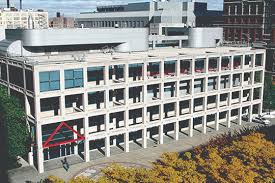
\includegraphics[width=\textwidth]{bern_dibner_lib.jpeg}
    \caption{Bern Dibner Library}
    \label{fig:bern_dibner}
\end{figure}

\end{document}
